\documentclass[a4,12pt]{scrreprt}

\usepackage{amsmath}
\usepackage{makecell}

\usepackage{graphicx}
\usepackage[T1]{fontenc}
\usepackage[ngerman]{babel}
\usepackage[colorlinks,
pdfpagelabels,
pdfstartview = FitH,
bookmarksopen = true,
bookmarksnumbered = true,
linkcolor = black,
plainpages = false,
hypertexnames = false,
citecolor = black] {hyperref}

\begin{document}

\title{Systhem Erde} \label{sec:Systhem Erde}
\maketitle

\tableofcontents
\newpage

\chapter{Erdaufbau}
\section{Elemente}
\subsection{Entstehung}
größtenteils als Nukleosynthese im Inneren eines Sterns\\
alter des Sonnensysthems: ca. 4,5 mrd Jahre\\
Häufigste Elemente: H;He;O;Si;Al;Fe\\

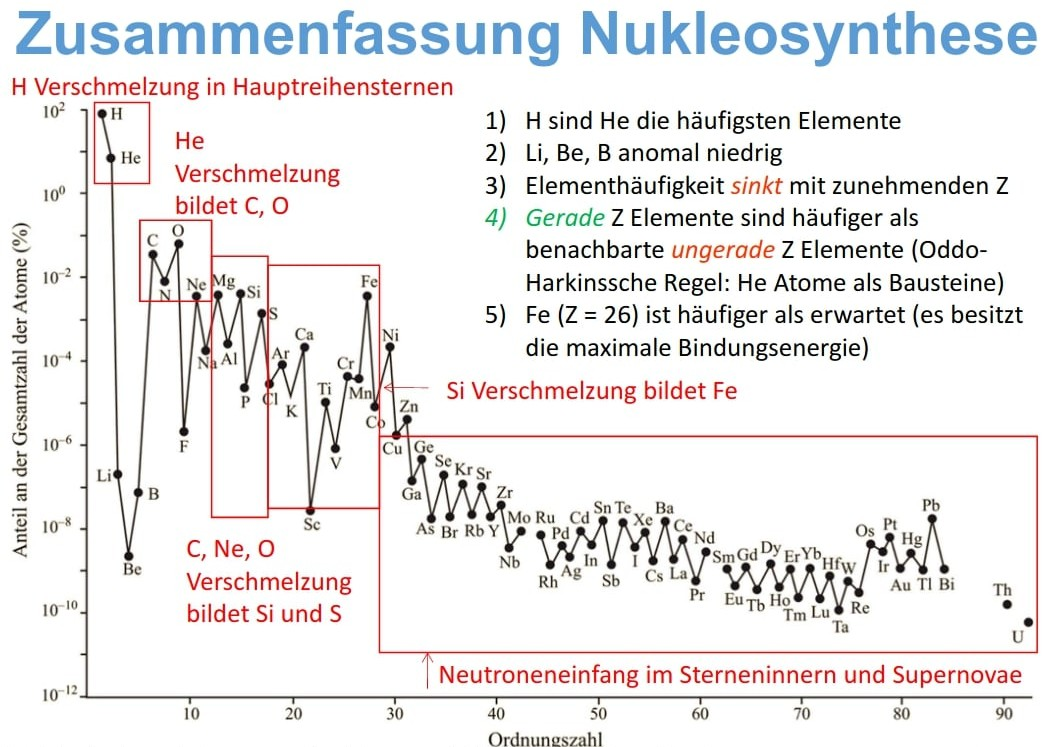
\includegraphics[width=1\textwidth]{/home/joni/Schreibtisch/Uni/Mittschriften/System_Erde/Bilder/Graph}\\

Elemente mit gerader Protonenzahl sind stabieler $\rightarrow$ Zick-Zack-Linie\\
Entstehung schwererer Elemente:
\begin{itemize}
\item R-Prozess: 1. schneller Neutronenfang z.B bei Supernova mit anschließendem $\beta$-Zerfall
\begin{itemize}
\item Neutronenfang ist schneller als der Kernzerfall
\item Tritt nur bei STernen mit mehr als 8 Sonnenmassen auf
\end{itemize}
\item S-Prozess: Neutronenfang von Kernschmelzen m inneren der Sonne mit anschließendem $\beta$-Zerfall
\begin{itemize}
\item Neutronenfang ist langsamer als der Zerfallsprozess
\item tritt bei Sternen mit weniger als 8 Sonnenmassen auf
\end{itemize}
\end{itemize}

\subsection{Ionen} \label{sec:Ionen}

Regeln für Ionenradien:\\
\begin{itemize}
\item Der Radius wächst mit der Ordnungszahl
\item Innerhalb eines Elements wächst der Radius mit der negativen Ladung\\ ($S^{2-}>S^{2+}$)
\item Der Radius nimmt mit der Koordinationszahl (Anzahl benachbarter Atome) zu
\item Bei seltenen Erden sinkt der Radius mit zunehmender Ordnungszahl
\end{itemize}

\subsection{Koordination der Atome im Molekül} \label{sec:Koordination der Atome im Molekül}

Wenn $\frac{2r_c}{2r_a} =$ (c = Kation, a = Anion)
\begin{enumerate}
\item 0,414	bis 0732, dann kann ein stabieles Oktaeda gebaut werden
\item 0,225 bis 0,414, dann kann ein stabiles Tetraeda gebaut werden
\end{enumerate}

\textbf{Druckkoordinationsregel}

\begin{itemize}
\item geringer Druck $\rightarrow \frac{2r_c}{2r_a}$ = gering $\rightarrow$ CN gering (CN = KoordinationsZahl)
\item hoher Druck $\rightarrow \frac{2r_c}{2r_a}$ = hoch $\rightarrow$ CN hoch
\end{itemize}

\newpage
\subsection{Silikate} \label{sec:Silikate}
$SiO_x$\\ 

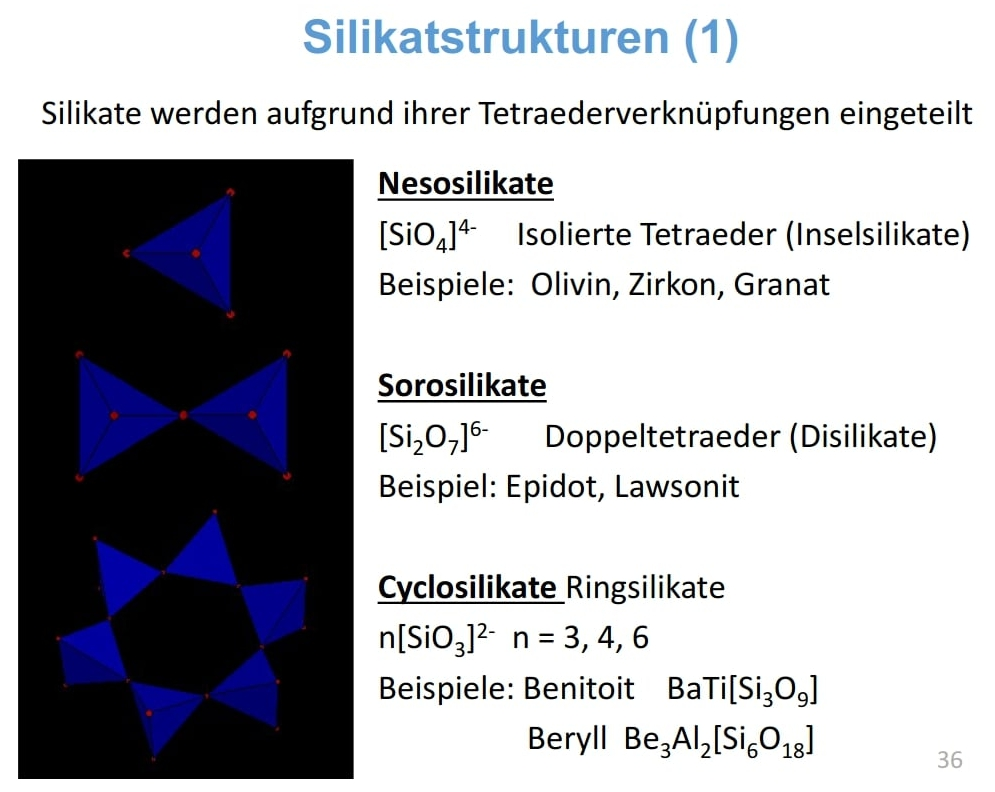
\includegraphics[width=0.8\textwidth]{/home/joni/Schreibtisch/Uni/Mittschriften/System_Erde/Bilder/Silikatstruktur1}

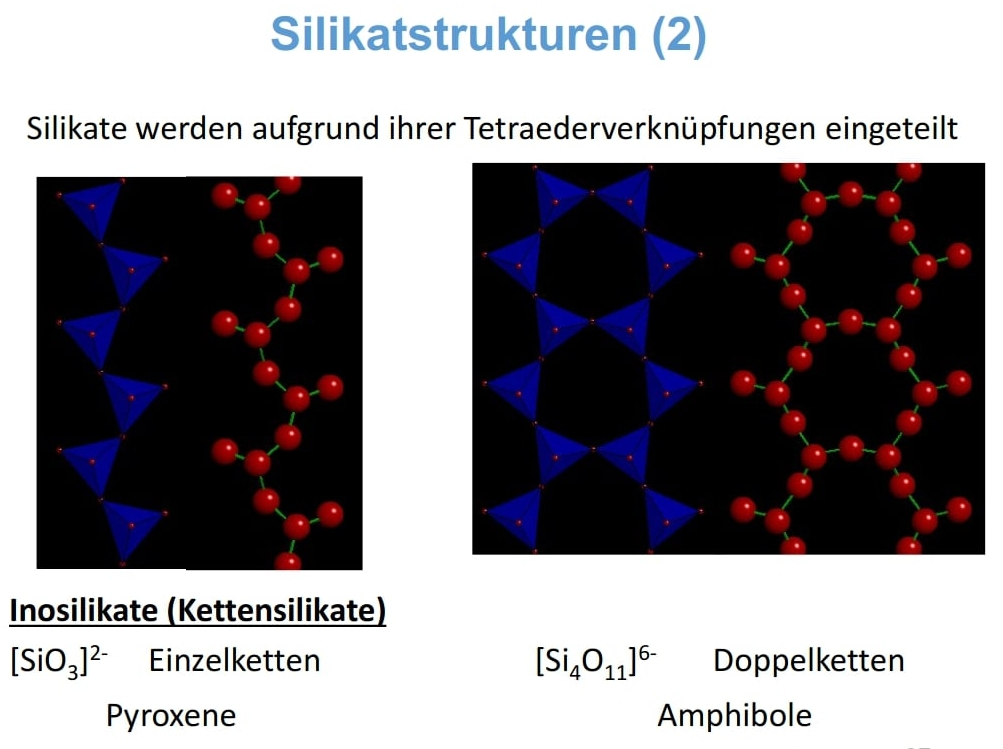
\includegraphics[width=0.8\textwidth]{/home/joni/Schreibtisch/Uni/Mittschriften/System_Erde/Bilder/Silikatstruktur2}\\

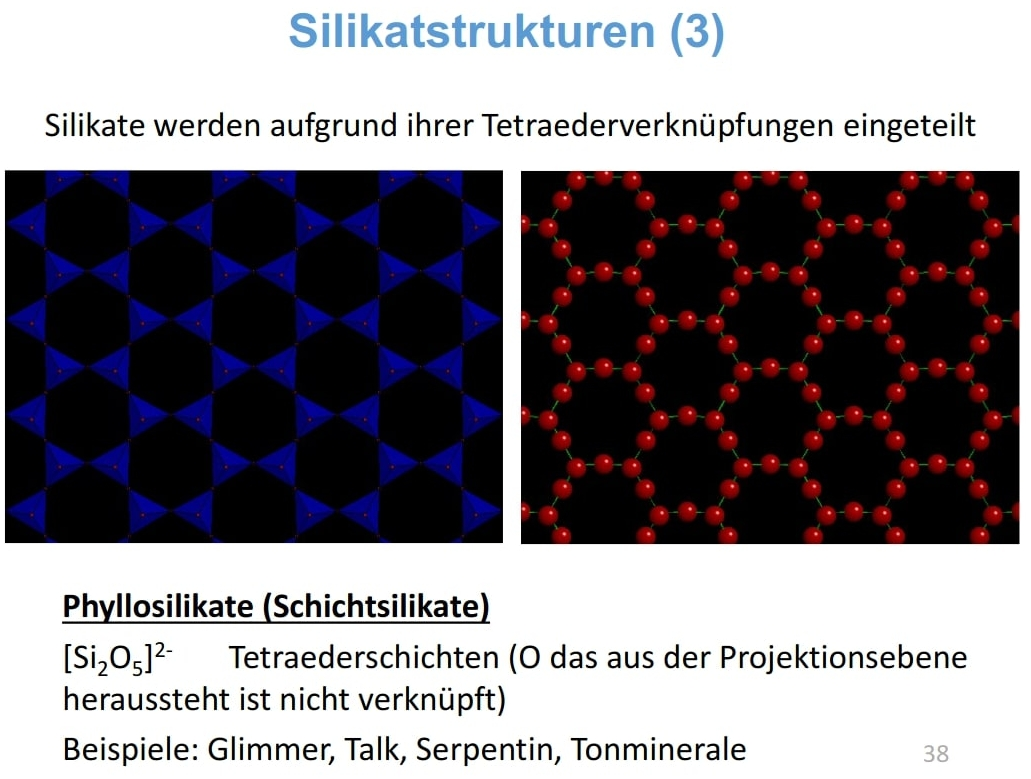
\includegraphics[width=0.8\textwidth]{/home/joni/Schreibtisch/Uni/Mittschriften/System_Erde/Bilder/Silikatstruktur3}\\

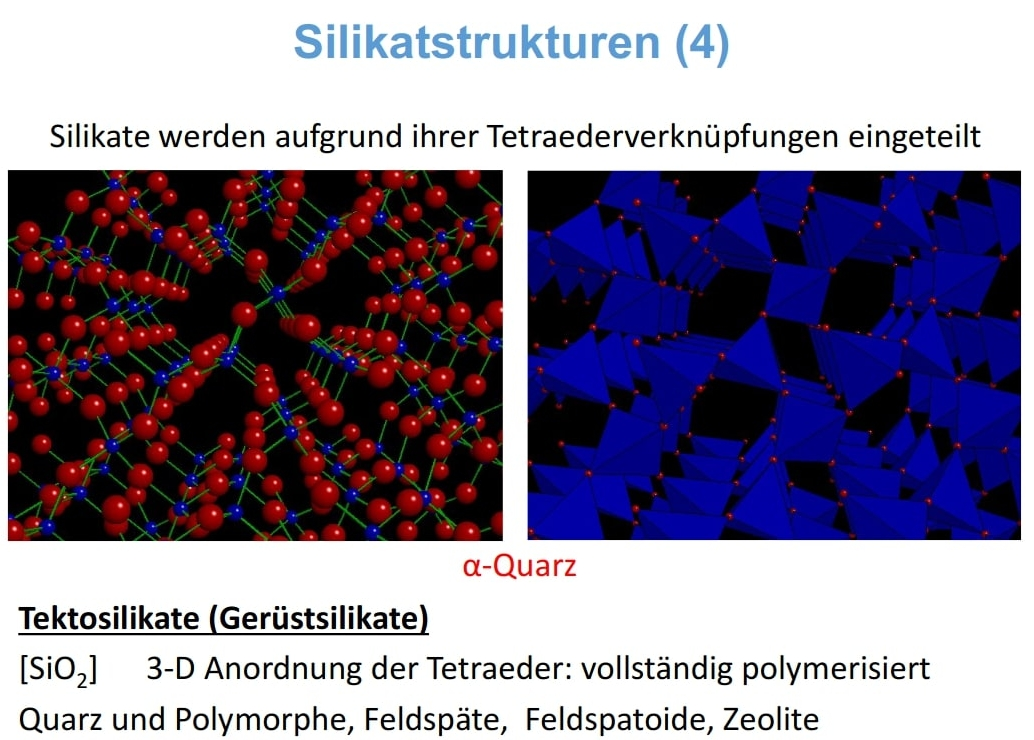
\includegraphics[width=0.8\textwidth]{/home/joni/Schreibtisch/Uni/Mittschriften/System_Erde/Bilder/Silikatstruktur4}\\

\newpage

\section{Entstehung des Sonnensystems}

\begin{itemize}
\item Bildung der Sonne aus protoplanetarem Nebel
\item Bildung einer Akkretionsscheibe aus den Überresten des Nebels
\begin{itemize}
\item entsteht durch den Drehimpuls des protosolaren Nebels
\end{itemize}
\item Durch Impakte in der Akkretionsscheibe entstehen Planetesimale
\item Revolution und Rotation von Sonne und PLaneten idR. gleich, da Impulserhaltung des Drehimpulses
\item Abweichungen in der Drehachse entstehen durch Impakte 
\item erste Verbindungen: CaAl-Verbindungen
\end{itemize}

\subsection{Orbitale Parameter der Erde} \label{sec:Orbitale Parameter der Erde}

3 Parameter verändern sich zyklisch:

\begin{itemize}
\item Exzentrizität: Abweichung von der Kreisbahn
\begin{itemize}
\item alle 100.000 Jahre
\item e schwankt zwischen 0,005 und 0,058 (e = 0 $\hat{=}$ Kreisbahn)
\end{itemize}
\item Obliquität: Schiefe der Erdachse
\begin{itemize}
\item alle 41000 Jahre
\item schwankt zwischen 22,1° und 24,5°
\end{itemize}
\item Präzession: Orientierung der Kreiselachse
\begin{itemize}
\item alle 26000 Jahre 
\end{itemize}
\end{itemize}

\section{Planeten} \label{sec:Planeten}
Merkur bis Mars überwiegend terristrische Planeten (überwiegend Gestein und Metall)\\
Jupiter bis Neptun Jovianische Planeten (überwiegend Helium und Wasserstoff)\\
Temperatur , Dichte und Silikate nehmen zur Sonne hin zu\\
Volatile Elemente ($H_2O,CO_2, CH_4,N_2$) nehmen ab\\

\section{Kometen}
Nukleus:\\

\begin{itemize}
\item fest
\item 10m bis 100km groß
\item besteht aus Eis und Gesteinskomponenten
\end{itemize}


Koma: Haarförmiger Schweif (Senkrecht zur Sonne stehende Streifen)
\begin{itemize}
\item durch Subblimation durch Sonnenwinde am Kometen freigesetzte Teilchen
\item entsteht, wenn der Komet auf bis zu 3-4 AE an die Sonne herankommt
\end{itemize}
Herkunft: Oortsche Wolke (Umlaufzeit  mehr als 200 Jahre)bzw. Kuipergürtel (Umlaufzeit weniger als 200 Jahre)

\section{Meteorite} \label{Meteorite}
Unterteilung in Eisen, Stein-Eisen, Stein Meteorite\\
Steinmeteorite können in Achondrite (weniger häufig) und Chondrite (häufig) unterteilt werden 

\subsection{Impakte} \label{Impakte}
Je größer der Impakt werden, desto komplexer werden die Krater	\\
Krater entsprechen denen einer Punktexplosion\
Einschläge produzieren immer einen runden Krater, außer der winkel ist sehr flach

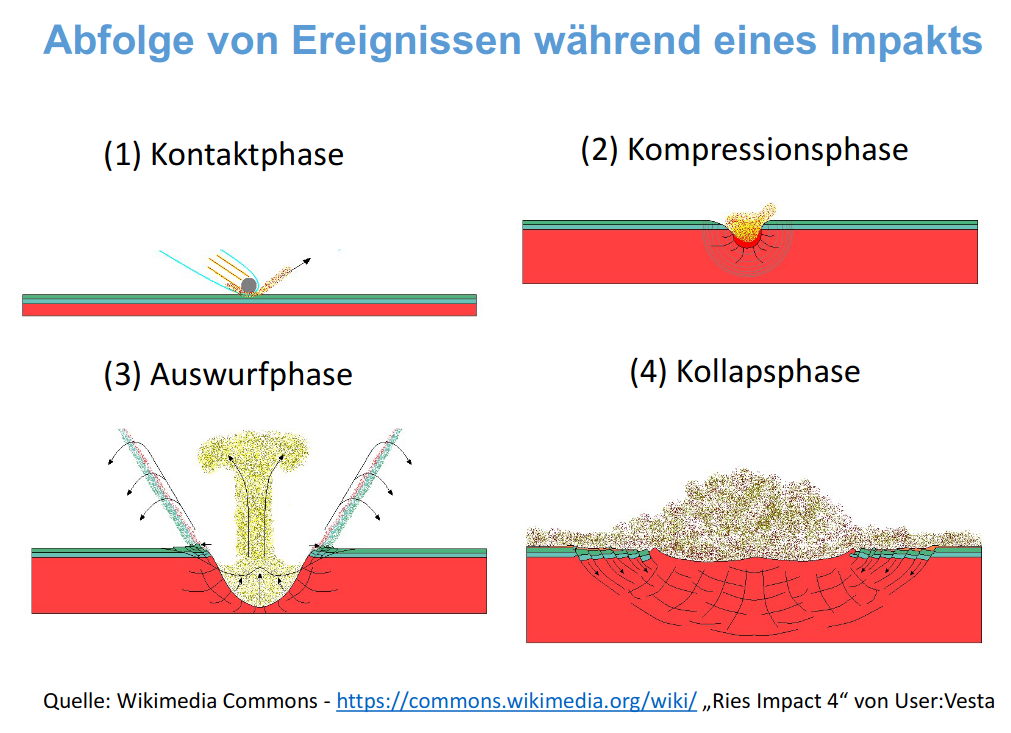
\includegraphics[width=0.8\textwidth]{/home/joni/Schreibtisch/Uni/Mittschriften/System_Erde/Bilder/Meteorimpakt}

\includegraphics[width=0.8\textwidth]{/home/joni/Schreibtisch/Uni/Mittschriften/System_Erde/Bilder/impaktstruktur}

\section{Atmosphäre und Leben} \label{Atmosphäre und Meteoriten}

\subsection{Leben} \label{Leben}
Faktoren, die die Entstehung von Leben begünstigen:\\
• Entfernung zur Sonne\\
• Akkretion(chemische Gradienten)\\
• Impakte\\
• Größe\\
• Atmosphäre (Treibhausgase)\\
• Magnetfeld zu Abschirmung energetischer Strahlung\\

\subsection{Atmosphäre}

Quellen:
\begin{itemize}
\item Entgasung
\item Verdunstung
\item Meteorite/Kometen
\item Stoffwechsel\\
\end{itemize}
Senken:
\begin{itemize}
\item Atmosphärische Flucht
\begin{itemize}
\item Entweichen der Oberen Atmosphärenschicht durch zuführung von Wärme, was dazu fürt, dass die Geschwindigkeit des Moleküls größer als die Fluchtgeschwindigkeit des Planeten wird
\end{itemize}
\item Ionisierung durch Sonnenwinde
\item große Impakte
\item Stoffwechsel
\end{itemize}

\section{Geschichte der Erde}

\href{file:/home/joni/Schreibtisch/Uni/Mittschriften/System_Erde/Bilder/Erdentstehung}{Präsi angucken}

\newpage
\section{Schalenbau der Erde}

\textbf{Kruste (1\%)}
\begin{itemize}
\item Ozeanisch:
\begin{itemize}
\item dünn (10km), jung (<160 Ma Jahre)
\item Zusammensezung: Basalt
\end{itemize}
\item Kontinental
\begin{itemize}
\item dick (30-60km), alt (Ga)
\item Zusammensetzung: Granodiorit
\\
\end{itemize}
\end{itemize}

\textbf{Mantel (87\%)}
\begin{itemize}
\item seismische Diskontiunition
\begin{itemize}
\item niedrige seismische Geschwindigkeiten im oberen Mantel
\item Zusammensetzung: Peridotid
\\
\end{itemize}
\end{itemize}

\textbf{Kern (12\%)}
\begin{itemize}
\item FE-reich, metallische Legierungen mit Ni, Si, S, O
\item Äußerer Kern Flüssig, innerer fest
\end{itemize}

\subsection{seismische Wellen}
\begin{enumerate}
\item Longitudinalwelle (P-Welle)
\begin{itemize}
\item Feder entlang der Höhe strecken und stauchen
\end{itemize}
\item Transversal (S-Welle)
\begin{itemize}
\item sinusförmig
\end{itemize}
\end{enumerate}

\subsection{Ausbreitungsgeschwindigkeit seismischer Wellen}

\includegraphics[width=0.8\textwidth]{/home/joni/Schreibtisch/Uni/Mittschriften/System_Erde/Bilder/seismische Geschwindigkeiten}\\

S-Wellen breiten sich in Flüssigkeiten nicht aus $\rightarrow$ Entstehung von Schattenzohnen

\section{Geothermie}

\textbf{Wärmequellen}
\begin{enumerate}
\item Insolation (Hauptwärmequelle)
\item Geothermie 
\begin{itemize}
\item Primordiale Wärme aus der Zeit der Akkredition und Differenzierung
\item radioaktiver Zerfall
\item Gezeitenreibung (sehr gering)
\end{itemize}
\end{enumerate}

\textbf{Wärmetransport}
\begin{enumerate}
\item Konduktion (Wärmeleitung)
\item Konvektion/Advektion
\item Strahlung
\end{enumerate}

\section{Magnetismus}

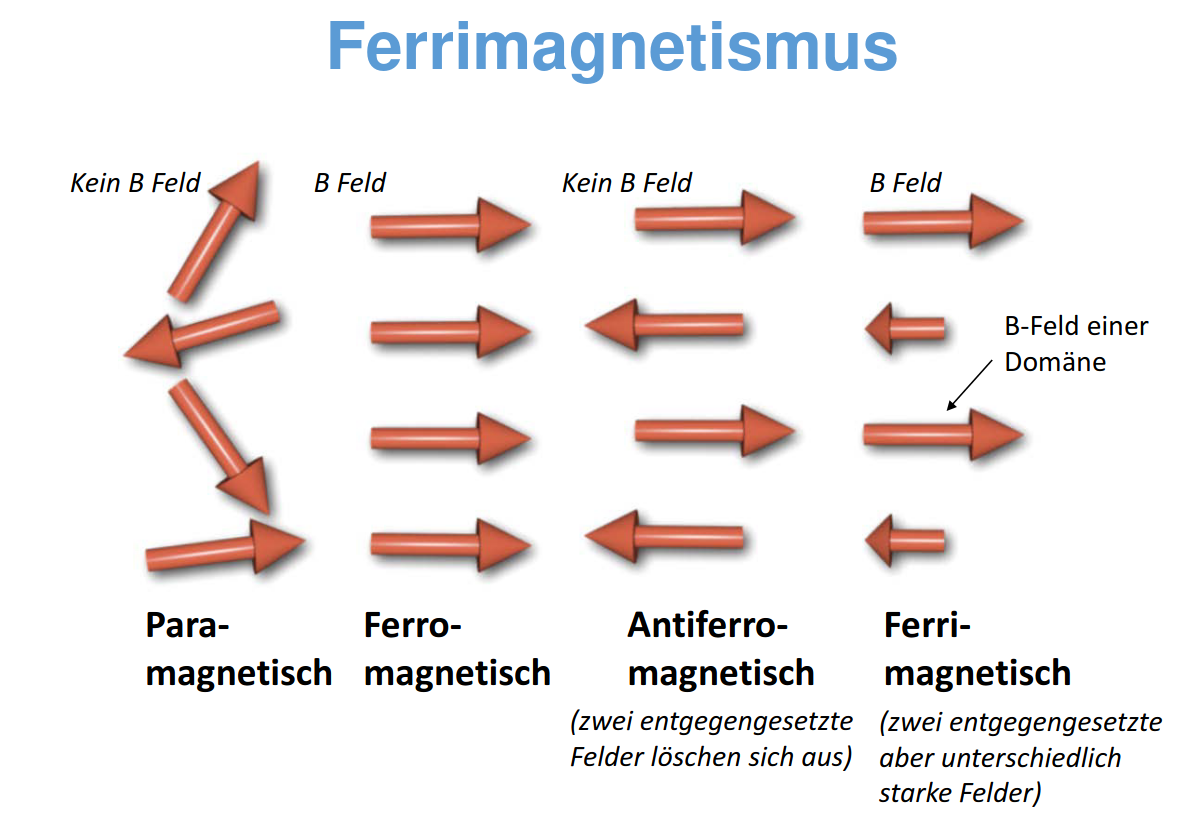
\includegraphics[width=0.8\textwidth]{/home/joni/Schreibtisch/Uni/Mittschriften/System_Erde/Bilder/Magnetfelder}\\

\section{Platenteltonik}
pro Theorie:
\begin{itemize}
\item Küstenlinien wie Puzzleteile
\item gleiche Fossilien auf unterschiwdlichen Kontinenten z.B Pflanzen, Krokodiele
\item Beobachtung der Gebirgsbildung: Steine können über weite Strecken horizontal berlappen
\item Ozeanische Kruste sehr jung
\begin{itemize}
\item Der Ozeanboden bildet sich neu an ozeanischen Spreizrücken
\end{itemize}
\end{itemize}

\subsection{Magnetisches Streifenmuster am Meeresboden}
\begin{itemize}
\item Larven treten am Meeresboden aus
\item wird abgeschrekt
\item Magnetische Ausrichtung friert im Gestein ein
\end{itemize}

\section{Lithosphärenplatten}
Lithosphäre: Kruste + oberer Mantel\\
starre/ feste Erde\\
\begin{enumerate}
\item Divergente Plattenbewegung()konstruktiv: Platten gehen auseinander $\rightarrow$ neue Ozeanische Lithosphäre\\
\item Konvergente Plattenbewegung(destruktiv): Platte gehen zusammen $\rightarrow$ Material wird eingeschmolzen\\
\item Transformstörungen Plattenbewegung (konservativ): entgegengesetzte Bewegungsrichtung (Händereiben) $\rightarrow$ nix passiert\\
\end{enumerate}

\subsection{Bewegung der Platten}
\begin{enumerate}
\item Rückenschub
\begin{itemize}
\item auftreibende Magma hebt die Kruste an
\end{itemize}
\item Plattenzug
\begin{itemize}
\item Eklogit zieht die Platte nach unten (hohe Dichte)
\end{itemize}
\end{enumerate}

\subsection{Typen von Plattengrenzen}

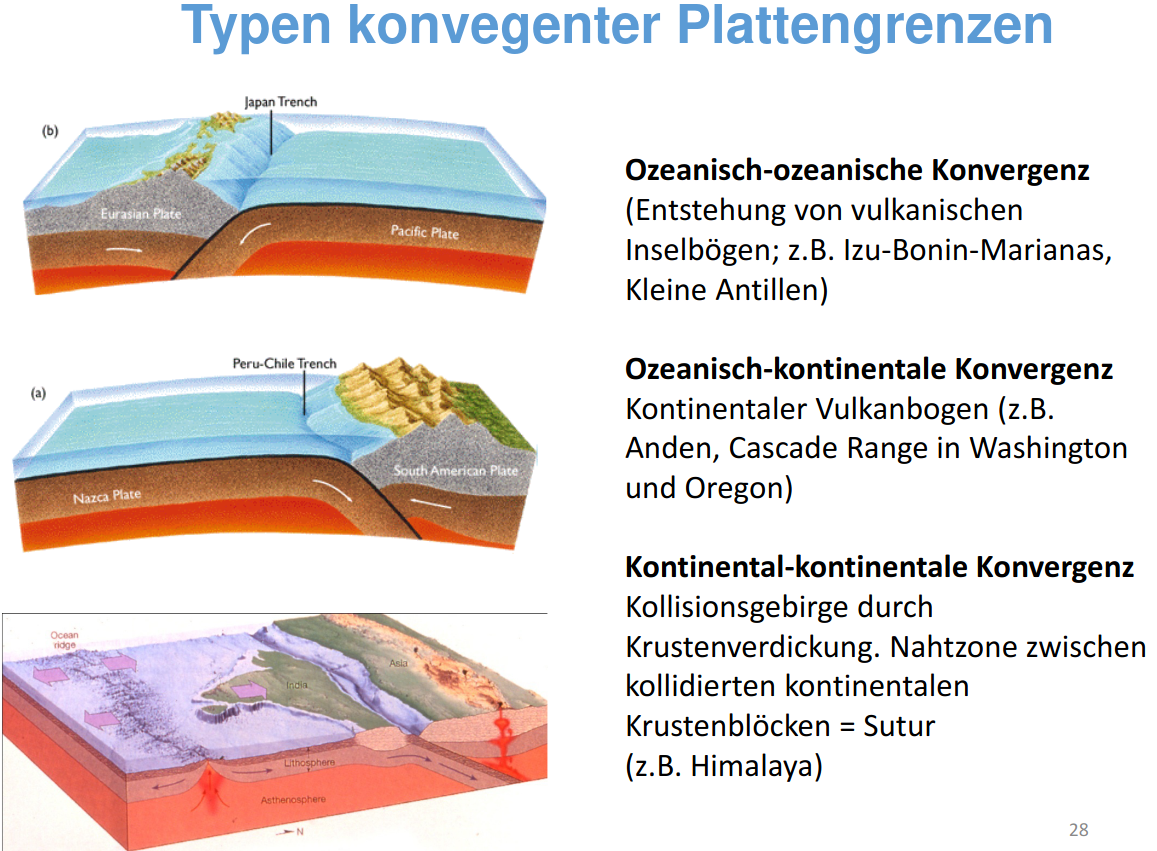
\includegraphics[width=0.8\textwidth]{/home/joni/Schreibtisch/Uni/Mittschriften/System_Erde/Bilder/destruktive Plattengrenzen}\\
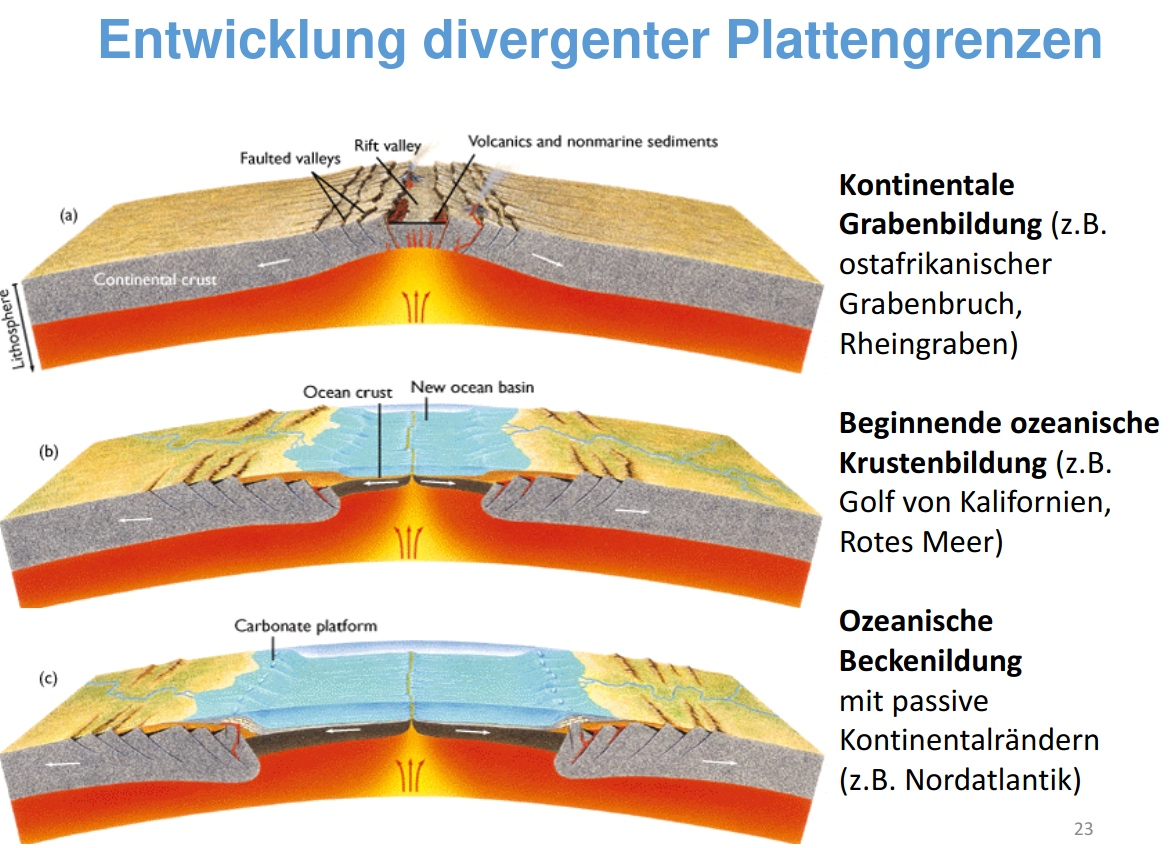
\includegraphics[width=0.8\textwidth]{/home/joni/Schreibtisch/Uni/Mittschriften/System_Erde/Bilder/konstruktive Plattengrenzen}\\

% was vergessen

\subsubsection{Blattverschiebung an Plattengrenzen}
Verschiebungsrichtung:
\begin{tabular}{ll}
dextral & nach rechts\\
sinistral & nach links\\
\end{tabular}

\section{Erdbeben und Plattengrenzen}

- Erdbeben können überall und jeder Zeit vorkommen\\
- nicht vorhersehbar aber Frühwarnungen möglich

\subsection{Präventionen}
\begin{itemize}
\item Nicht auf störungen bauen
\item auf nachwirkungen vorbereiten z.B Feuer, Wassermangel, 
\item Erdbeben töten nicht; herabstürzende Bauten töten
\end{itemize}

\subsection{Ursache}
- Durch Verschiebung an Plattengrenzen erzeugte Spannungen lösen sich sprungartig\\

\section{Erdbebenlokation}
- Triangulation von verschiedenen Messstationen\\
- An einer Messstation kann die Entfernung vom Erdbeben durch die unterschiedlichen Geschwindigkeiten der S und P-Welle bestimmt werden. 

\section{Herdflächenlösung}

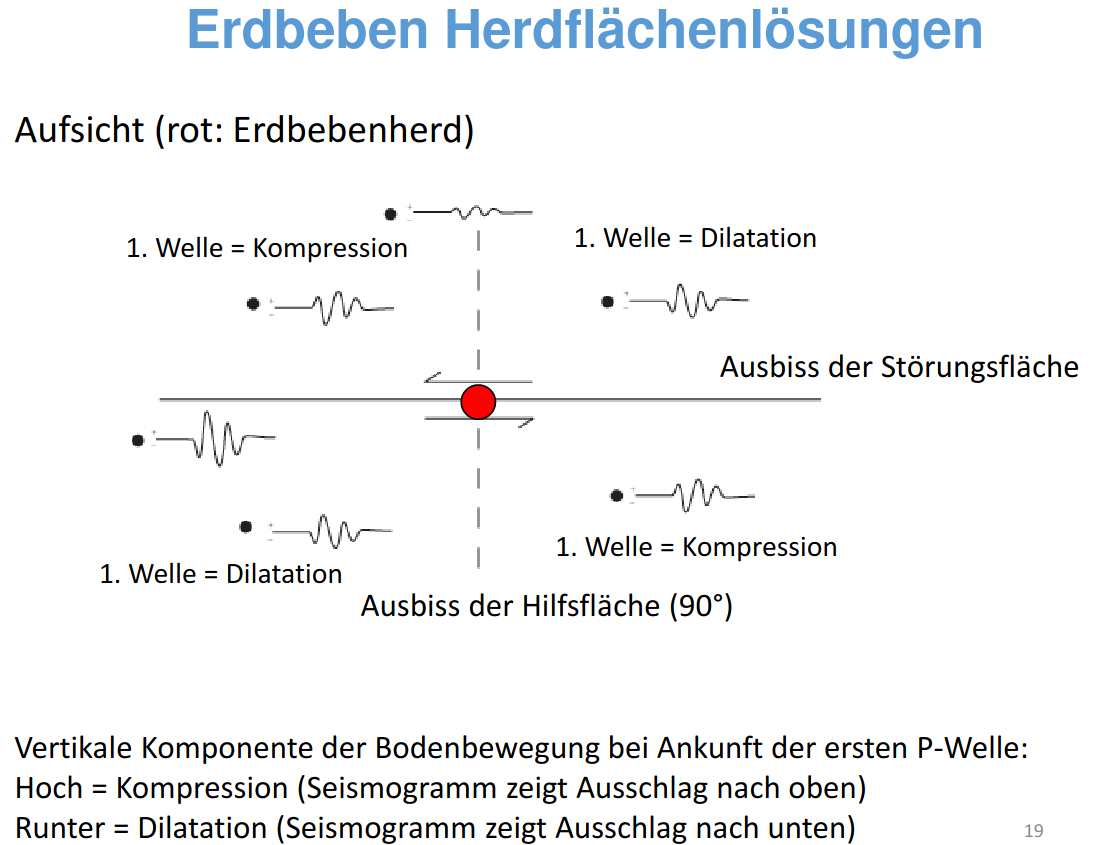
\includegraphics[width=0.8\textwidth]{/home/joni/Schreibtisch/Uni/Mittschriften/System_Erde/Bilder/Herdflächenlösung}\\

Beachball (Entsteht, wenn man die Flächen von Dilatation weis und von Kompression schwarz färbt) ist nicht eindeutig\\

\includegraphics[width=0.7\textwidth]{/home/joni/Schreibtisch/Uni/Mittschriften/System_Erde/Bilder/Störungsgeometrien}\\

\section{Erdbebenstärken}
- verschiedene Gesteine verhalten sich beim gleichen Erdbeben unterschiedliche (Liquefaktion z.B nur bei sedimenten, nicht Gesteinen)

\subsection{Momenten-Magnetudenskala}

Erdbeben mit $M_W$ +1 hat im Vergleich zu $M_W$
\begin{enumerate}
\item 10-mal stärkere Maximalerschütterung
\item 3,3-mal größeren Versatz und Dauer
\item 32 mal weitere Rissfläche/höhere Energie in Form von seismischen Welen
\end{enumerate}

\subsection{Verhalten beim Erdbeben}
-Drop\\
-cover\\
-hold\\
\section{vulkanismus}

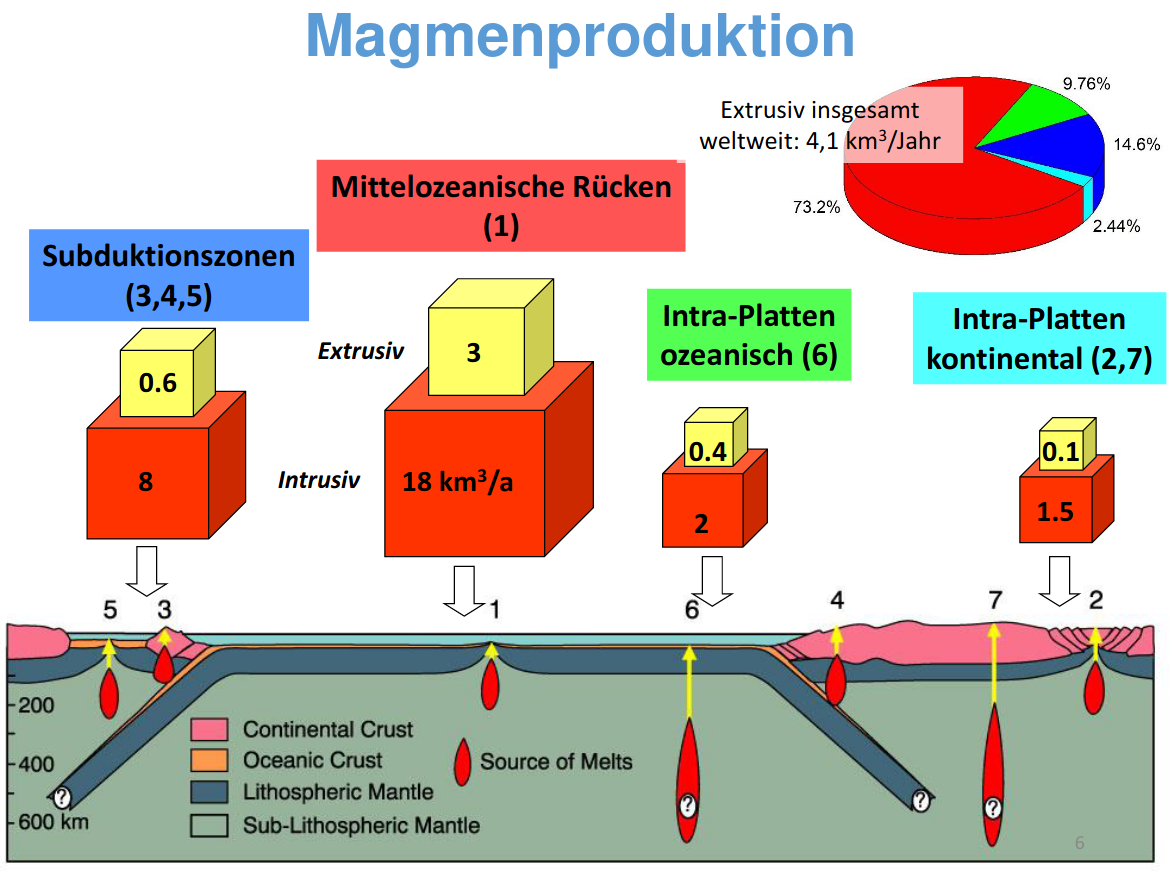
\includegraphics[width=0.7\textwidth]{/home/joni/Schreibtisch/Uni/Mittschriften/System_Erde/Bilder/Magmenproduktion}\\

Ursache von Vulkanismus ist Konvektion\\
Eigenschaften von Magmen:\\
besteht aus Kristallen, Gasfasen und flüssigem Gestein\\
\subsection{(Silikat-)Schmelzen}
\begin{tabular}{l|ll}
Kategorie & Rhyolithische Schmelze & basaltische Schmelze\\
\hline
gekennzeichnet durch & wenn hohe Konzentration von vernetzter $SiO_2$ & wenn niedrige Konzentration vernetzter $SiO_2$\\
Dichte & weniger Dicht & Dicht\\
Viskosität & sehr hoch (Erdussbutter) & eher niedrig (Kechup)\\
Eruption & fließt einfach ab & eher explosiv\\
\end{tabular}\\
\\
Explosion in rhyolithischen Schmelzen, durch "Explosion", da Gasbildung (Blasenbildung) in der Schmelze durch Druckentlastung.\\
\\
\textbf{Vulkantypen:}\\
\begin{tabular}{l|l}
Maare & entstehen, wenn eine Explosion unter der Erde geschiet, wenn Wasser auf Magma trifft.\\
Stratovulkane & heufig als Kette, entstehen durch Lagen von erkalteter Magma. heufig explosieve Eruption\\
Lavadome & $SiO_2$ reiche, entgaste Laven. z,B Ryolith\\
Calderen & bilden sich durch Einbruch von Deckenschichten über ausgedehnten Magmenreservoiren\\
\end{tabular}\\
\\
\textbf{Vulkanische Gefährdung}\\
\begin{tabular}{l|l}
Lava & 100tem bis 1km\\
Pyroklastische Ströhme & 1km bis 10km\\
Lahar (Schlammströme) & 10km\\
Vulkanische Asche & 10km bis 1000km\\
vulkanische Gase & global\\
\end{tabular}

\section{Ozeanische Kruste}
\subsection{mittelozeanische Rücken}
\begin{itemize}
\item 65.000 km lange Kette divergenter Plattenränder
\item 70\% des Gesammten Vulkanismus
\end{itemize}

\subsection{Tiefseebergketten}
\begin{itemize}
\item Inselketten, die durch vulkanische Aktivität an Hot Spots entstehen
lineare Kette, die die ozeanische Plattenbewegung nachzeichnen
\end{itemize}

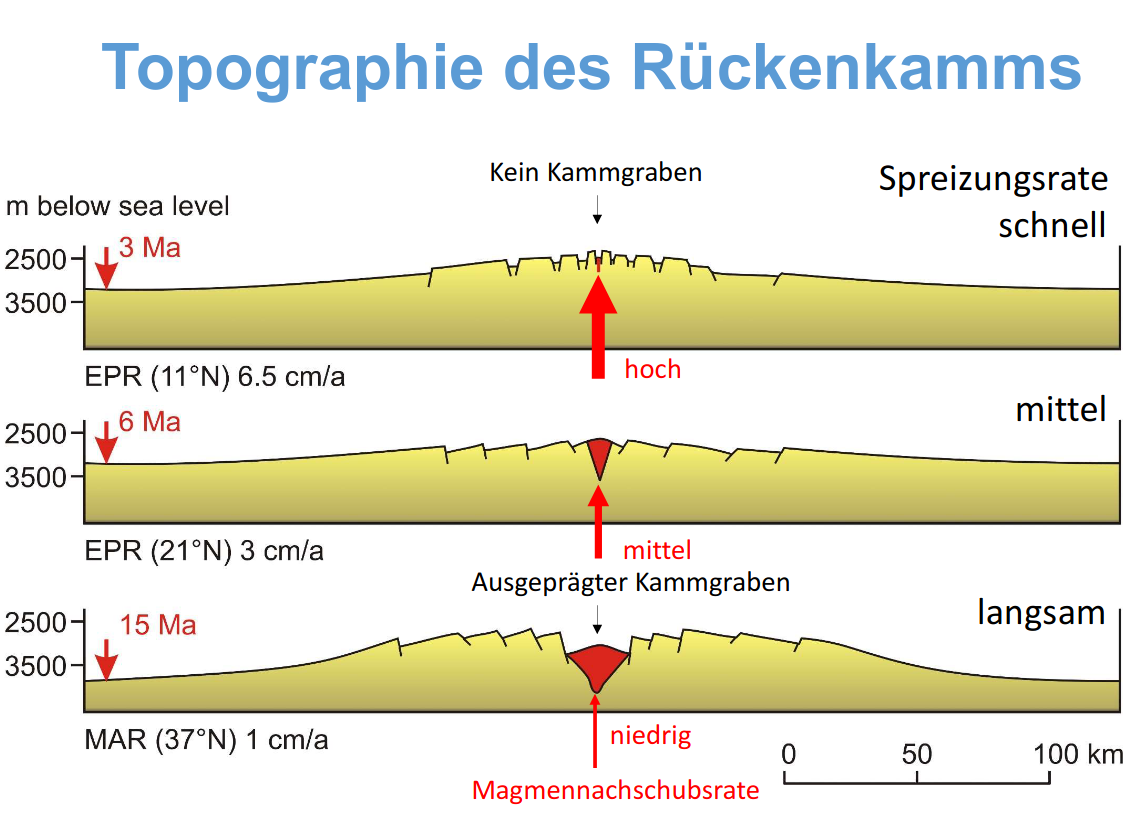
\includegraphics[width=0.75\textwidth]{/home/joni/Schreibtisch/Uni/Mittschriften/System_Erde/Bilder/Spreizungsraten}\\

\subsection{submariner Vulkanismus}
\begin{itemize}
\item überwiegend effusiv
\item hoher Wasserdruck verhindert Gasentmischung
\item Bildung von Pillowbasalten
\end{itemize}

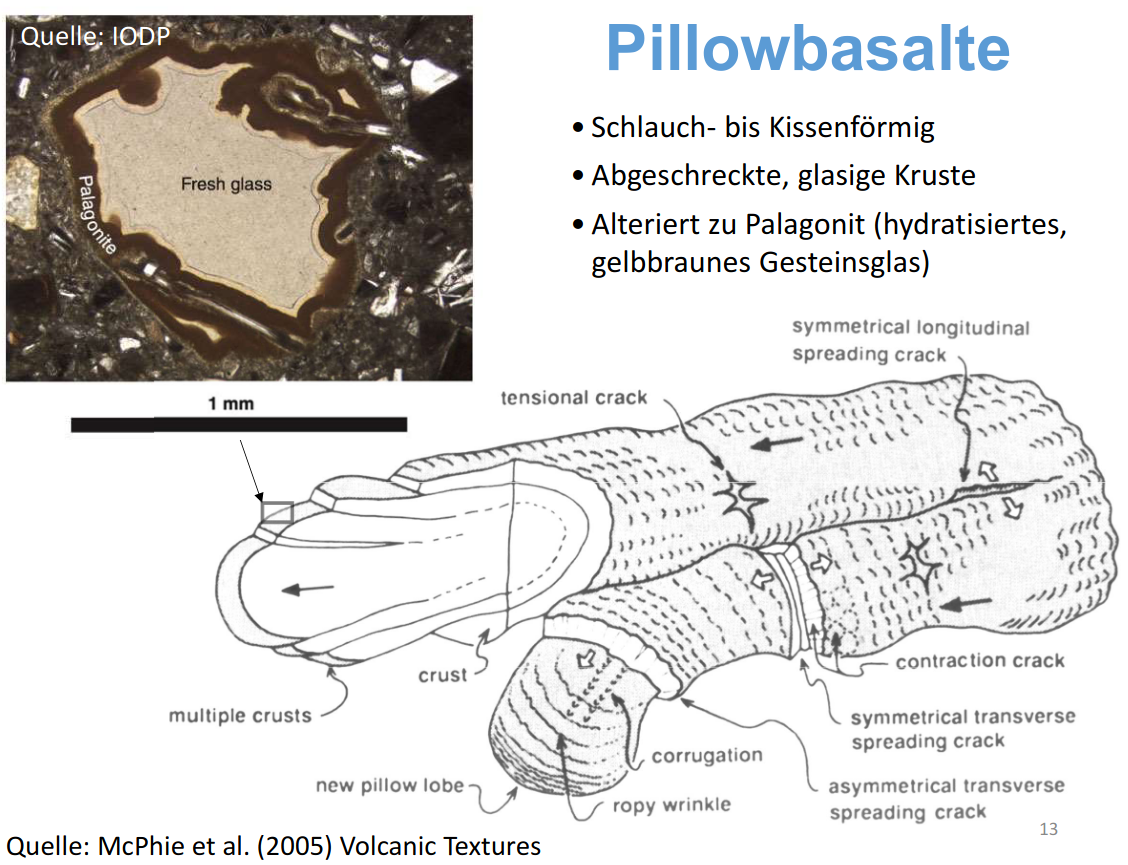
\includegraphics[width=0.75\textwidth]{/home/joni/Schreibtisch/Uni/Mittschriften/System_Erde/Bilder/Pillowbasalt}\\

\section{Aufbau der ozeanischen Kruste}
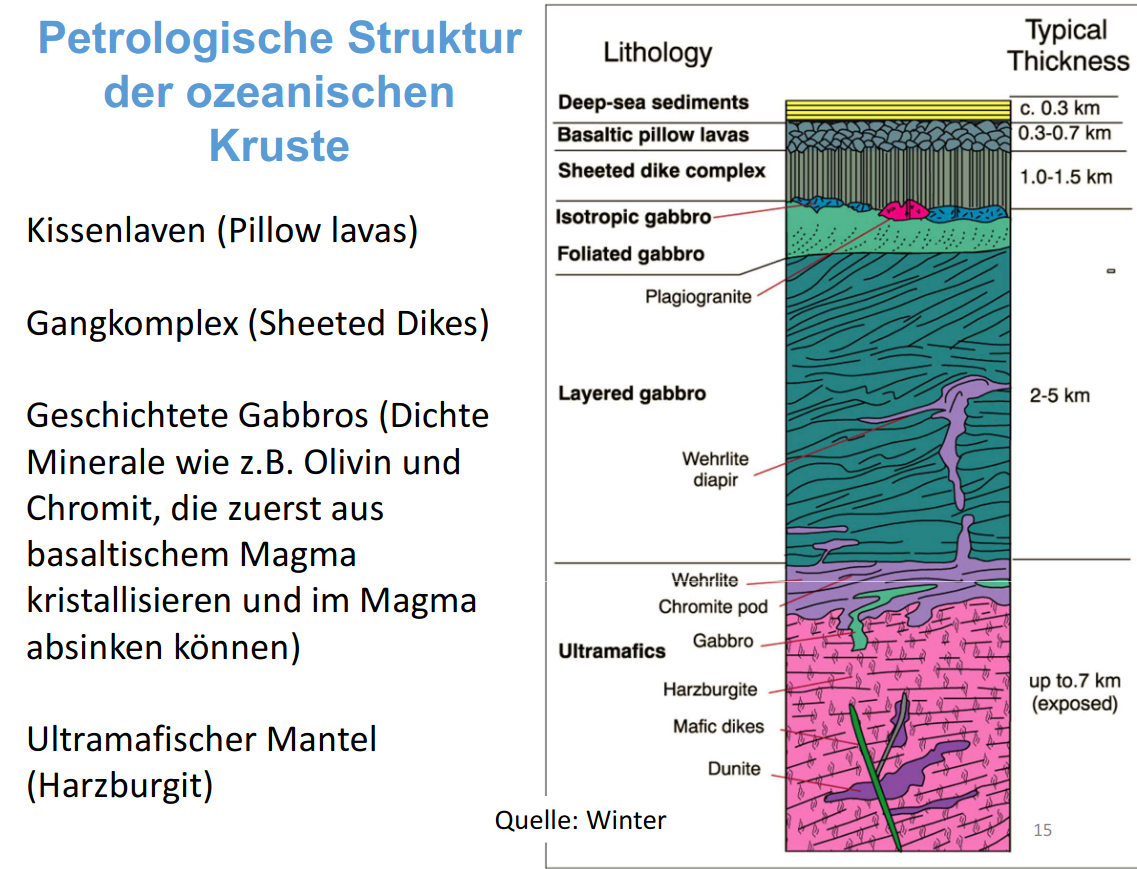
\includegraphics[width=0.8\textwidth]{/home/joni/Schreibtisch/Uni/Mittschriften/System_Erde/Bilder/Aufbau Ozeanische Kruste}\\

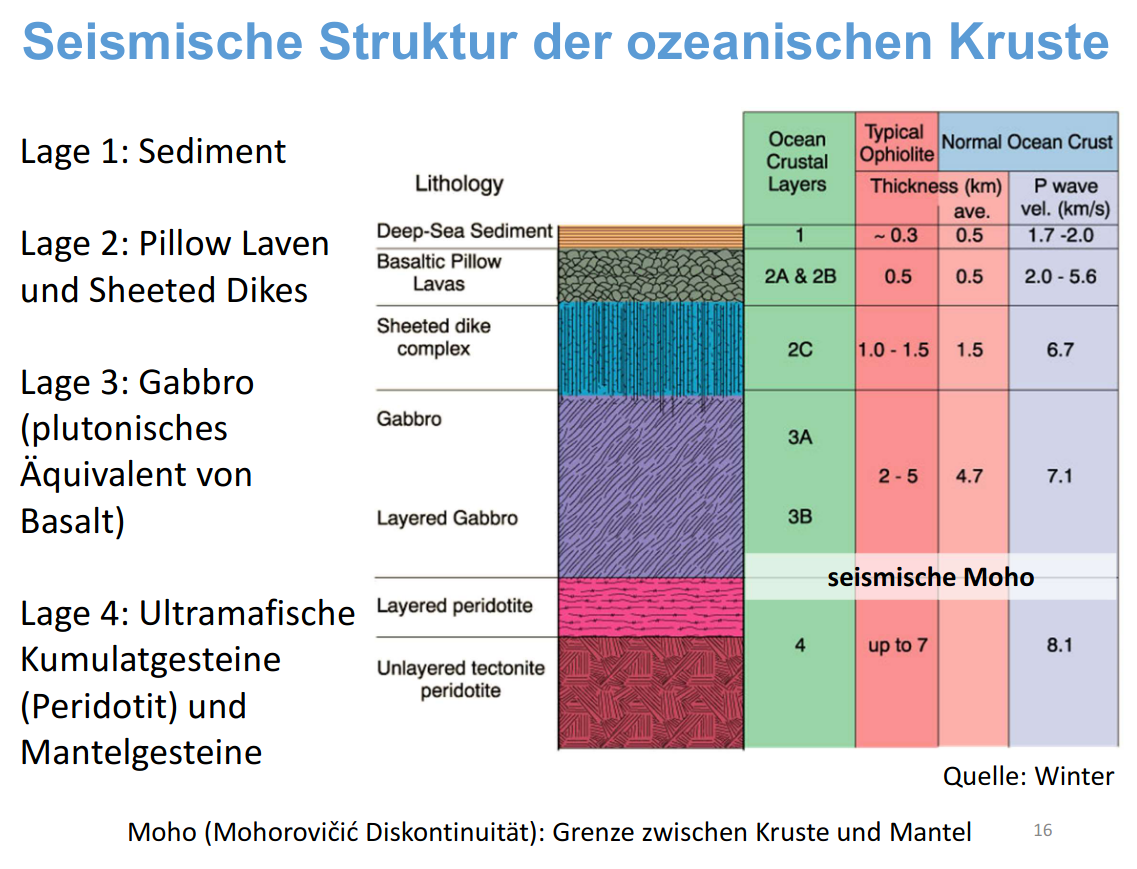
\includegraphics[width=0.8\textwidth]{/home/joni/Schreibtisch/Uni/Mittschriften/System_Erde/Bilder/Aufbau Ozeanische Kruste2}\\

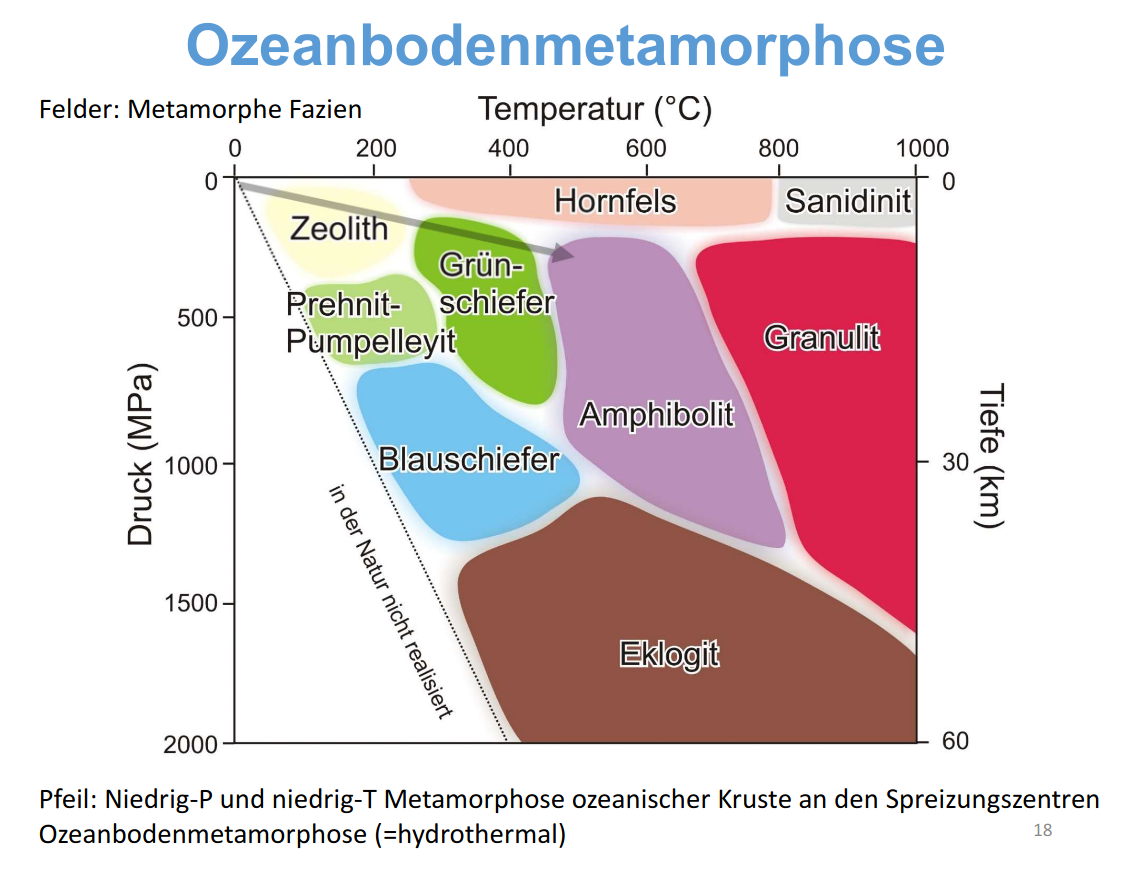
\includegraphics[width=0.8\textwidth]{/home/joni/Schreibtisch/Uni/Mittschriften/System_Erde/Bilder/Ozeanbodenmethamorphose}\\

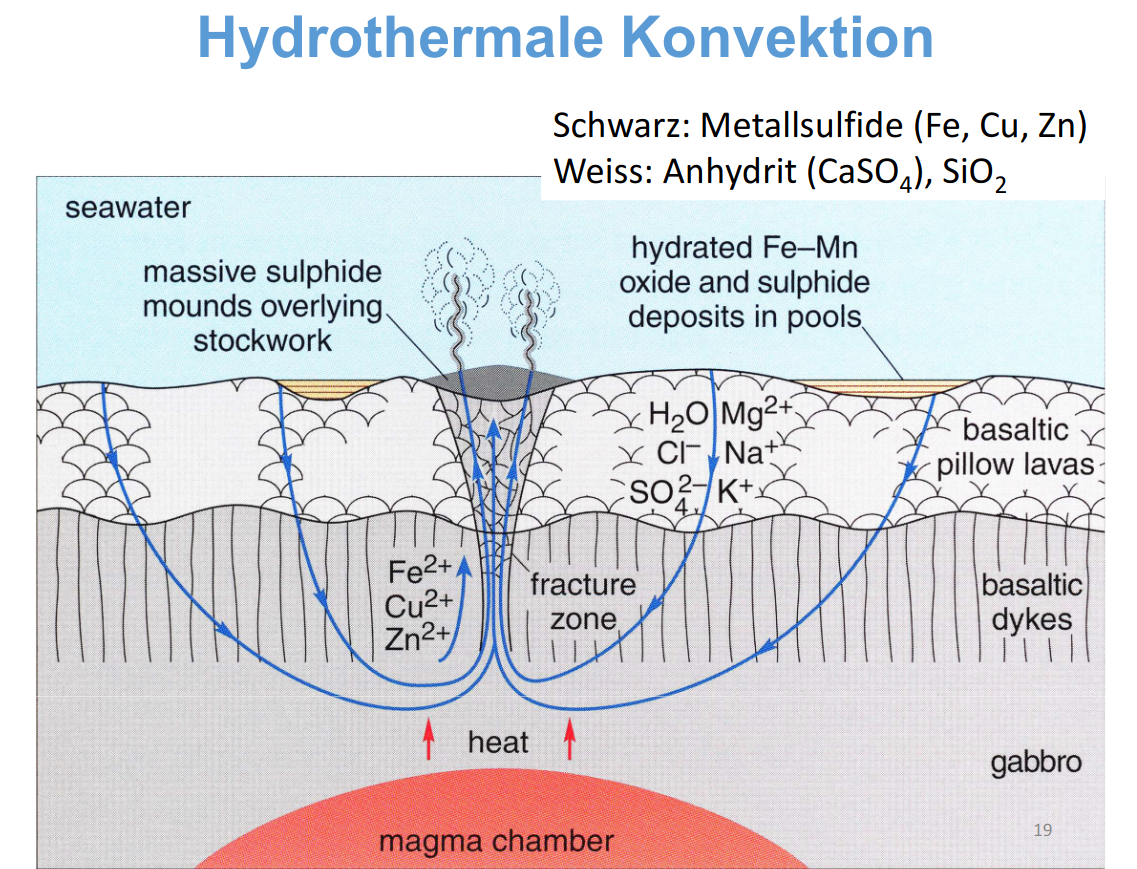
\includegraphics[width=0.8\textwidth]{/home/joni/Schreibtisch/Uni/Mittschriften/System_Erde/Bilder/Hydrothermale Konvektion}\\


%Mittschrift fehlt
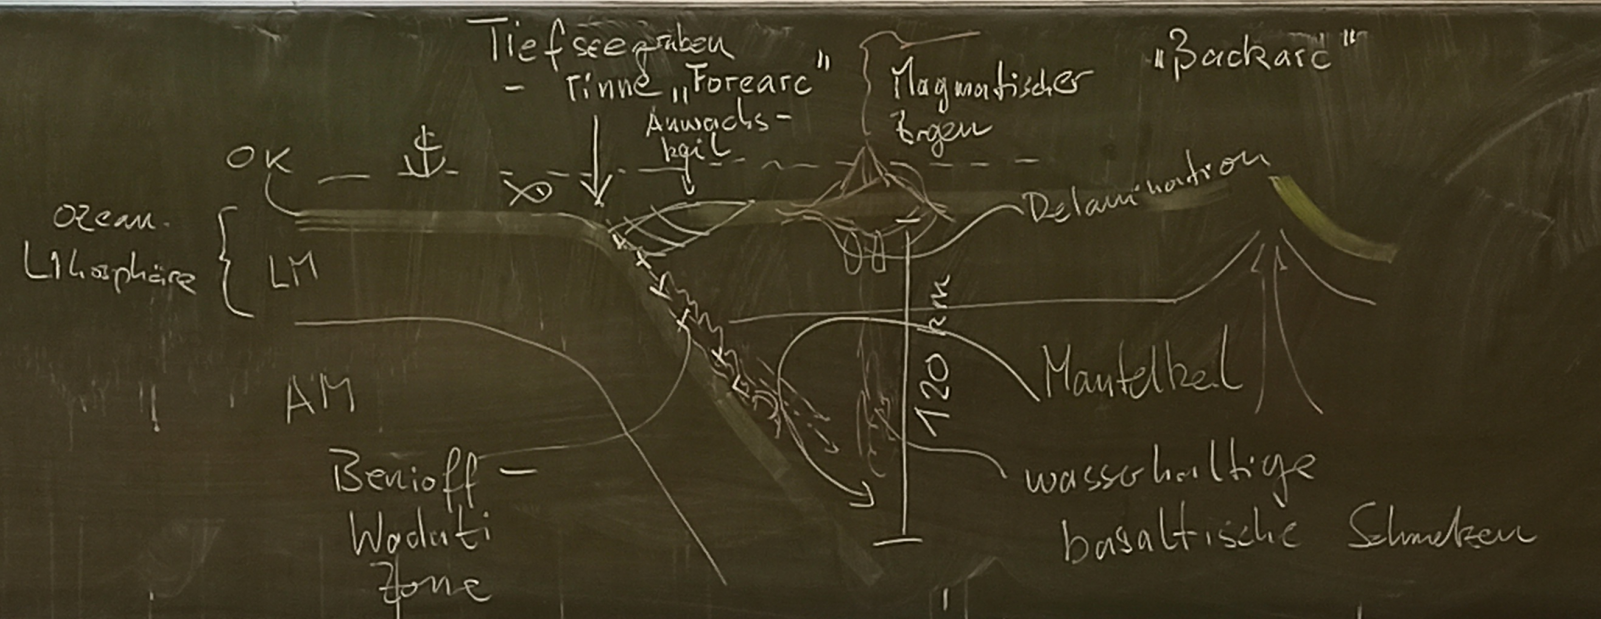
\includegraphics[width=0.8\textwidth]{/home/joni/Schreibtisch/Uni/Mittschriften/System_Erde/Bilder/subduktion}\\

\section{Gebirgsbildung}
- bilden sich durch plattentektonischen Prozessen, wobei das Relief durch das wechselspiel von endogenen bzw exogenen Prozessen bestimmt wird.\\
-sehr kurzlebige Gebilde (x 10 mio Jahre)\\

\section{Metamorphose}

-bei niedrigen Temperaturen brechen die Minerale
-bei hohen Temperaturen dehnen sich die Minerale spaghettiartig
\subsection{Metamophe Gesteine ohne Schieferung}
-Kristalle strukturieren sich neu (Rekristallisation) meist größer
\subsection{Matamorphe Gefüge in geblätterten Mineralen}
richten sich senkrecht zur Hauptspannungsrichtung aus $\rightarrow$ Schieferung

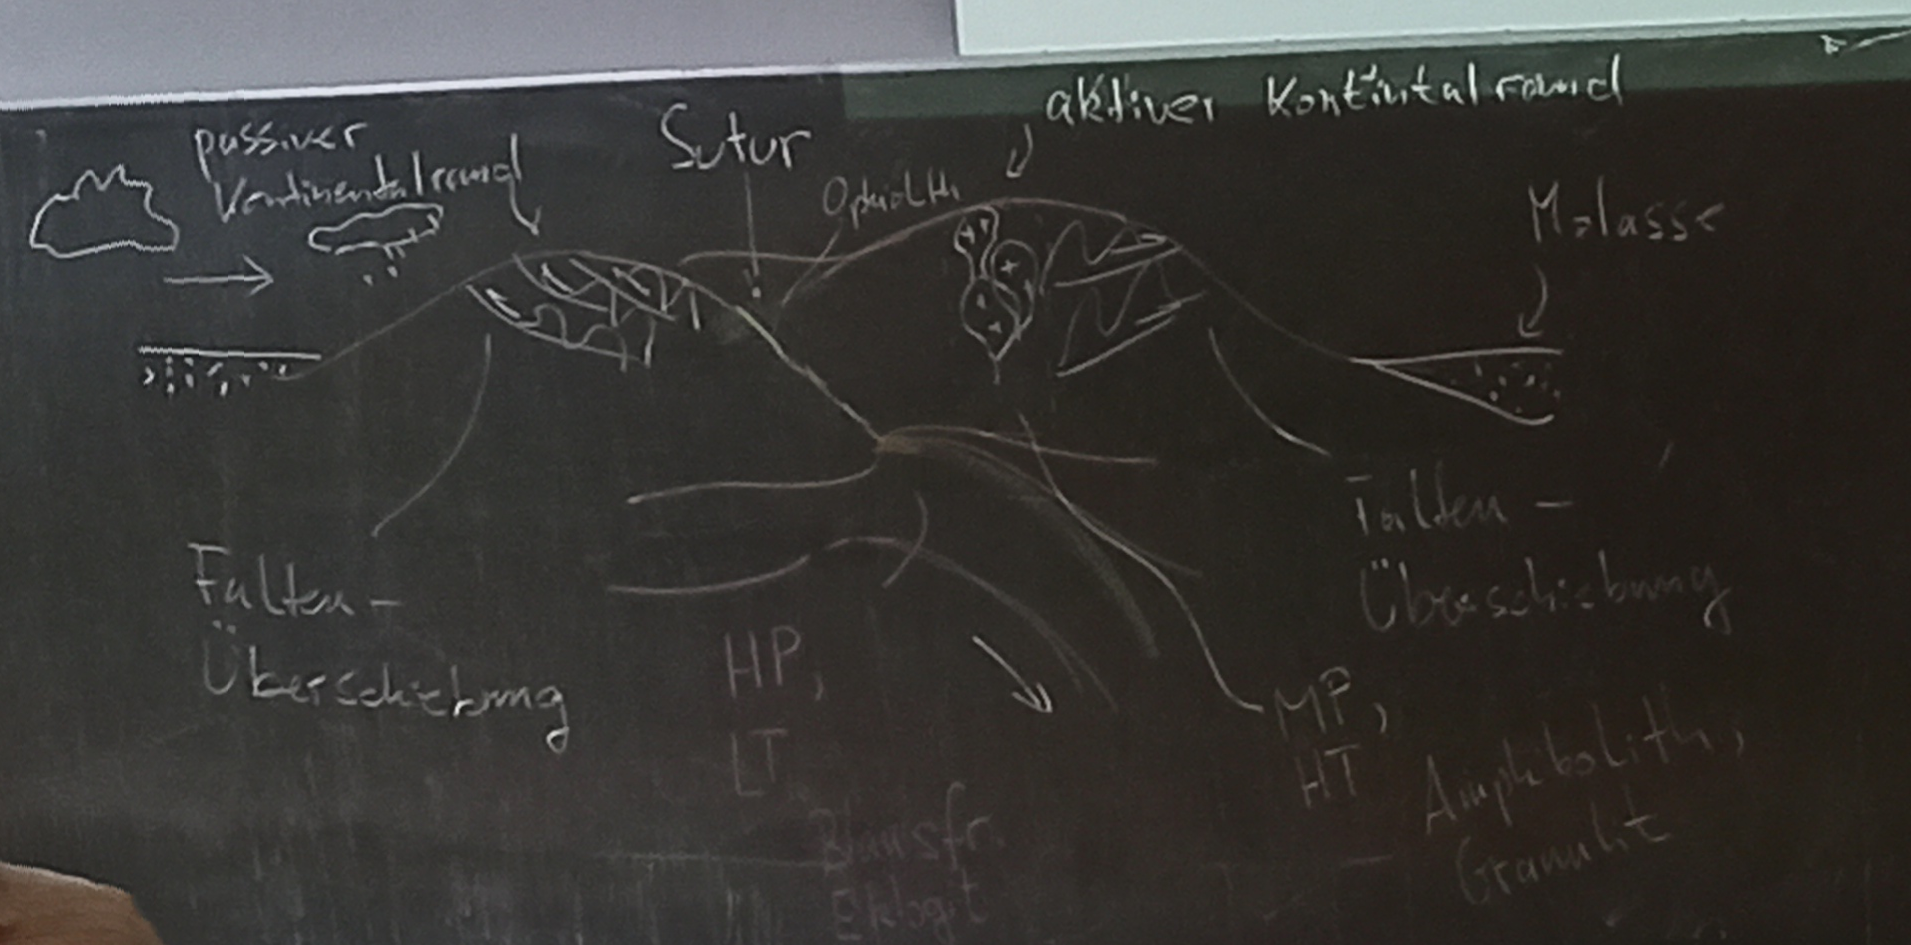
\includegraphics[width=0.8\textwidth]{/home/joni/Schreibtisch/Uni/Mittschriften/System_Erde/Bilder/Vls1}\\


\section{Verwitterung}
\subsection{Gesteinsverwitterung}
\textbf{Physikalischen Verwitterung}
\begin{itemize}
\item Wurzelsprengung
\item Thermische Ausdehnung
\item Abspaltung
\item Frostsprengung
\end{itemize}

\subsection{chemische Verwitterung}

\textbf{lösen von bestimmten Mineralen aus dem Gestein}\\

\begin{enumerate}
\item Kalkstein/Mamor (Calcit)\\
$CaCO_3 + 2H^+ \rightleftharpoons Ca^{2+}+H_2O+CO_2$
\item Mafische Gesteine (Fe/Mg-reiche Gesteine)
$MgFeSiO_4-4H^+\rightleftharpoons	 Mg^{2+}+Fe{2+}+2H_2O+SiO_4$\\
$2Fe^{2+\frac{1}{2}O_2+3H_2O}\rightleftharpoons 2FeO(OH)+4H$
\item granitische Gesteine (Feldspäte)\\
$2NaAlSi_3O_8+2H^++H_2O\rightleftharpoons Al_2Si_2O_5(OH)_4+4SiO_2+Na^+$
\end{enumerate}

\subsection{Bodenverwitterung}
\textbf{Aufbau}

\begin{itemize}
\item Oberboden\\
-Humus, Edaphon (Bodenflora- und Fauna)
\item Intermediäre Horizonte sind durch Eluation (Auswaschung feiner Bodenpartikel), Auslaugung(Verarmung an löslichen Komponenten) undAkkumulation(Einwaschen von Tonmineralen und Fe-Oxidbildung =Verbraunung) gekennzeichnet
\end{itemize}

\begin{itemize}
\item Molisol: Dunkler Oberboden, reich an Mumus\\
entwickelt sich nin Grasländern\\
\item Aridisol: dünner bis fehlender Oberboden, Wechsel des Mineralgehalts zyklisch durch ausspühlung und aufsaugen durch kapilarkäfte\\
\item Oxisol: tiefgründig verwittert, enthalten überwiegend unlösliche Komponenten, sehr arm an Rohstoffen\\
\end{itemize}

\subsection{Bodenerosion}
\begin{itemize}
\item durch Wind
\item durch Wasser\\
Protection: Terrassen anlegen oder Rillen senkrecht zum Berghang anlegen
\item Bodenversalzung
\end{itemize}

\section{Massenbewegung und Erosion}
\begin{itemize}
\item je grobkörniger das Material, desto höher die Reibung zwischen den Objekten, desto höher der Schüttwinkel
\end{itemize}
\subsection{Klassifikation von Massebewegungen}
\begin{tabular}{lllll}
Nennung & Material & Bewegungsart & Geschwindigkeit\\
Steinlawinen/Bergstürze & Gestein & Fallen/rutschen & schnell\\
\makecell Muren (Schlamm und\\ Schuttströhme) & Wasser und Gestein & fließen/rollen & schnell
Kriechen/Solifluktion & \makecell Böden, z.T \\ größeres Gestein & \makecell Hebung und Senkung \\ des Bodens & langsam\\
\end{tabular}

\chapter{Sedimente und Erdgeschichte}

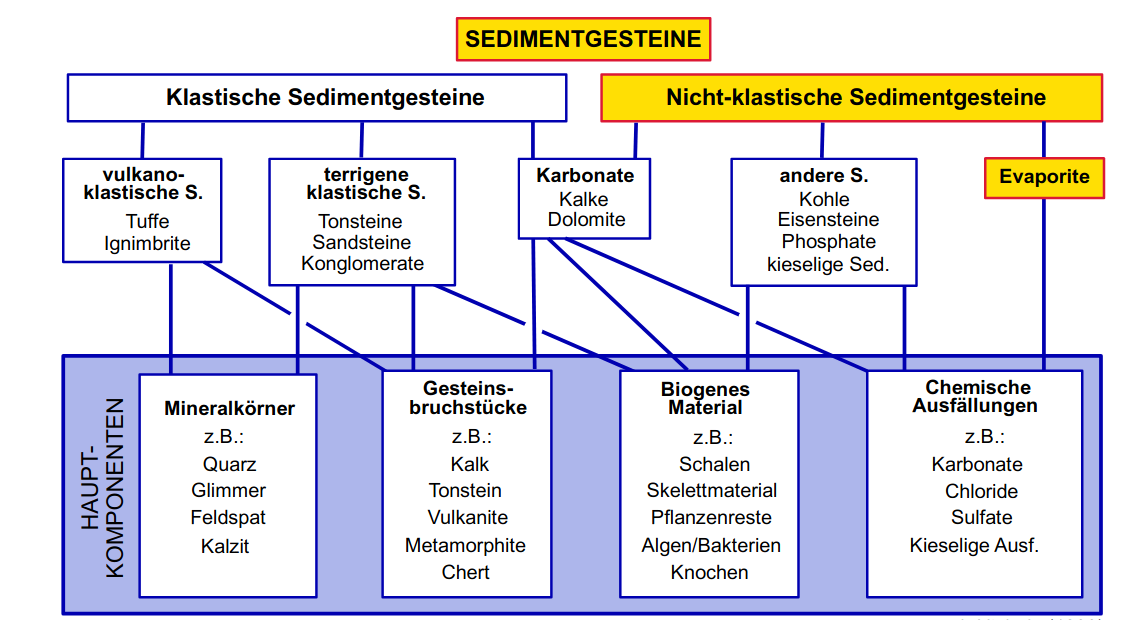
\includegraphics[width=0.8\textwidth]{/home/joni/Schreibtisch/Uni/Mittschriften/System_Erde/Bilder/Klassifikation Sedimente}\\
\section{terigene klastische Sedimente}
Ton <2$\mu$m
Schluff 2-63 $\mu$m
-setzt sich zum größten Teil aus Quarz, aber auch aus feldspäten, Muskovit Kalzit oder Eisenoxiden\\

Transport 1 in Suspension (Wasser)\\
Transport 2 Wind --> Löss\\

\subsection{Löss}
hohe Standfestigkeit\\
Entstehung: Winde verlagern Sediment an spezielle Orte\\

\section{vulkano-klastische Sedimente}
Quelle: Vulkane\\
$\rightarrow$ an geotektonische Settings gebunden z.B Subduktionszonen, Hotspots oder Mittelozeanische Rücken\\

Unterscheidung durch Korngröße (wie Vulkanoide)\\
Zusammensetztung: Mineralkörner, Gesteinsfragmente, Glas und Bimsstein\\

\section{biiogene Karbonate}

Herkunft: aus Korallen oder Schalentieren $\rightarrow$ Karbonatschlämme\\
hauptsächlich in den niederen bis mittleren Breiten zu finden, weil CCD-Fläche:\\
in tieferne Wässern ist mehr $CO_2$ enthalten (in Wasser Kohlensäure) was $CaCO_3$ auflöst\\


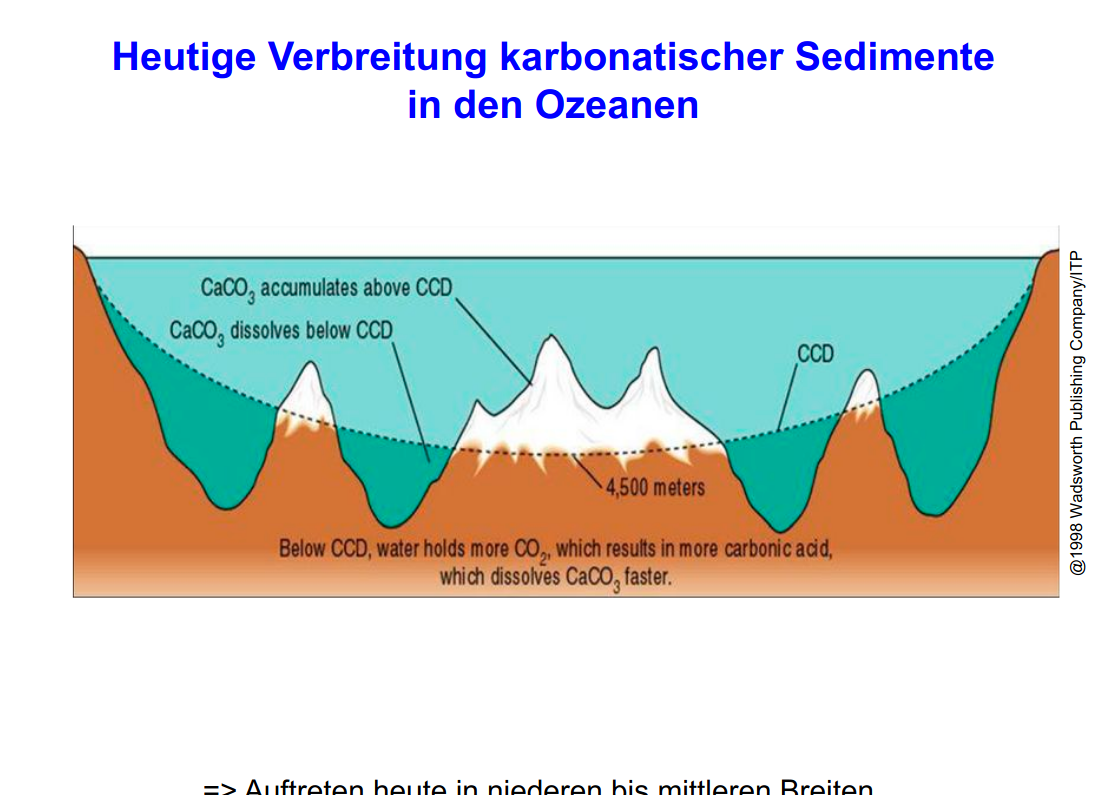
\includegraphics[width=0.8\textwidth]{/home/joni/Schreibtisch/Uni/Mittschriften/System_Erde/Bilder/CCD}\\

\newpage
Karbonate bestehen aus: \\

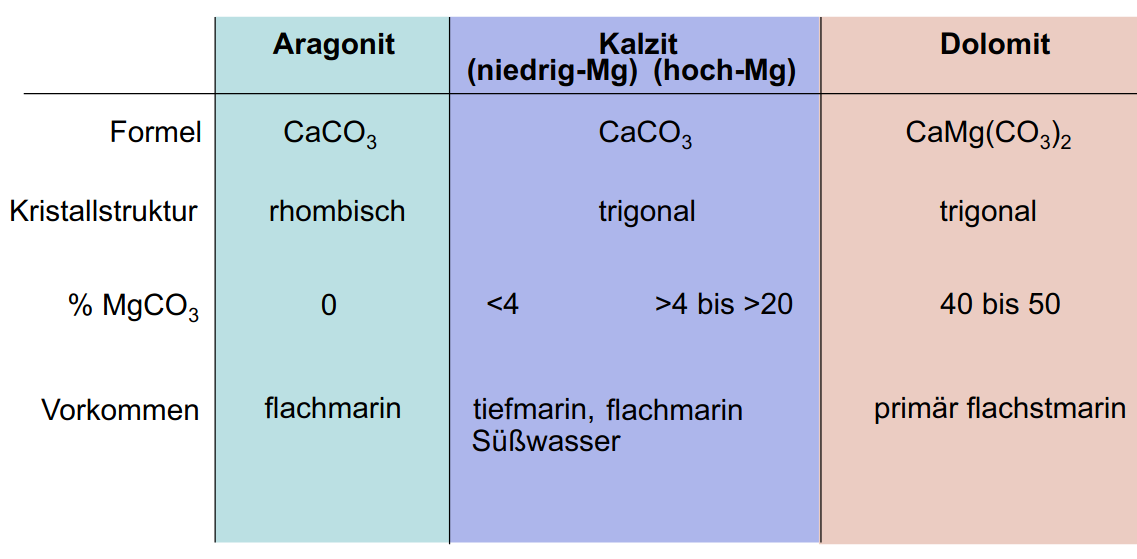
\includegraphics[width=0.8\textwidth]{/home/joni/Schreibtisch/Uni/Mittschriften/System_Erde/Bilder/Kalzitbestandteile}\\

\section{Evaporite}
Entstehung: durch chemische Ausfällung durch Verdampfung\\
mit dem Grad der Eindampfung steigend:
\begin{itemize}
\item Karbonate (Kalzit, Dolomit)
\item Sulfate (Gips, Anhydrit)
\item Salze (K-Salze, Halite)
\end{itemize}

\section{andere Sedimente und Kohle}
Entstehung aus: Humus(in Böde), Torf(Mooren und Sümpfen), Sapropel(Seen/Meer)\\
wird zu Schwarzschiefer(>2\%)/Kohle(>65\%)\\

\subsection{Schwarzschiefer im Meer}
Bedingung: anoxische Bedingungen im Wsasser ($\rightarrow$ keine Durchmischung)





\end{document}